%************************************************
\chapter{Design and implementation}\label{ch:design}
%************************************************

% Estructura:
% +Design
%  -Architecture design: delegation, computation offloading, duality User/SC + Engine
% 


In this chapter we will describe the process for defining how a constrained IoT device may be integrated in a system like P2ABCE. We will also describe the PoC implementation carried out to test a realistic deployment.

\section{Design}

In this section we will define how an IoT device may be integrated in the P2ABCE architecture, being totally compatible with any other system using P2ABCE, addressing the power and memory constrains many IoT devices face.

We decided to use P2ABCE with the Idemix as its Engine, because it is officially supported by the Idemix Library, it has the most up-to-date implementation, as we saw in the state of the art, and adds capabilities to Idemix like the Presentation Policies, or interoperability with U-Prove, not available without the P2ABCE project.

Our main goal is to make an IoT device capable to act as a User or Verifier in the P2ABCE architecture. For this, the device should be able to \textbf{communicate} with the Verifier or Prover with which it is interacting, manage the P2ABCE complex \textbf{XML schemas} transmitted, and perform the \textbf{cryptographic operations} required.

The communication between actors depends on each IoT scenario, it can be achieved with many existing standard solutions, e.g. an IP network, a Bluetooth M2M connection, RF communication, etc.

Our real concerns are, on one side, parsing the XML data, based on the P2ABCE's XML schema, that specifies the data artifacts created and exchanged during the issuance, presentation, revocation and inspection of pABCs; and on the other side, the cryptographic operations, that involve the use of secret keys, stored privately in the IoT device.

After the analysis done in the previous sections to the P2ABCE architecture, emphasizing that the logic of smart cards gathers the cryptographic operations independently from how the data is exchanged between P2ABCE actors. 

Using the \textit{computation offloading} technique to our scenario, our design consists on implementing the smart card logic inside the IoT device, keeping secure our master key and credentials, and for the rest of the P2ABCE system, if the device can not run the complete Engine, it may delegate to a server running it, indicating how to send APDU Commands to the \textit{IoT smart card}.

Even in the case we were to implement all P2ABCE inside an IoT device, we would have to implement the support for software smart cards, to keep the secret inside the IoT device. Therefore, we can begin implementing the smart card logic inside the IoT device, and later, if the device resources admit it, other components of the P2ABCE project.


\hfil

Computation offloading is not new to IoT deployments. For example, IPv6 involves managing 128 bits per address and other headers, and many IoT scenes only need to communicate inside a private network, making only the last 64 bits in an address relevant. To reduce that overhead, instead of IPv6 they use 6LoWPAN to compress packets and use smaller address sizes. To communicate a 6LoWPAN with the Internet or other networks, the IoT devices delegate the networking workload on a proxy that can manage the 6LoWPAN and IPv6 stacks. In the scope of consumer devices, smart bands or watches can install applications, bit many of them delegate on the user's phone to accomplish their task.

Therefore, the IoT device now has a \textbf{duality} in its functions, because it is the User that starts any interaction with other actors, and it's also the smart card that a P2ABCE server must ask for cryptographic operations. It can also be seen as a \textbf{double delegation}. The IoT device delegates on the external P2ABCE server to manage the protocol, and the P2ABCE server delegates on the IoT, acting now as a smart card, for the cryptography.

\subsection{System architecture}



\begin{figure}[bth]
	\begin{center}
		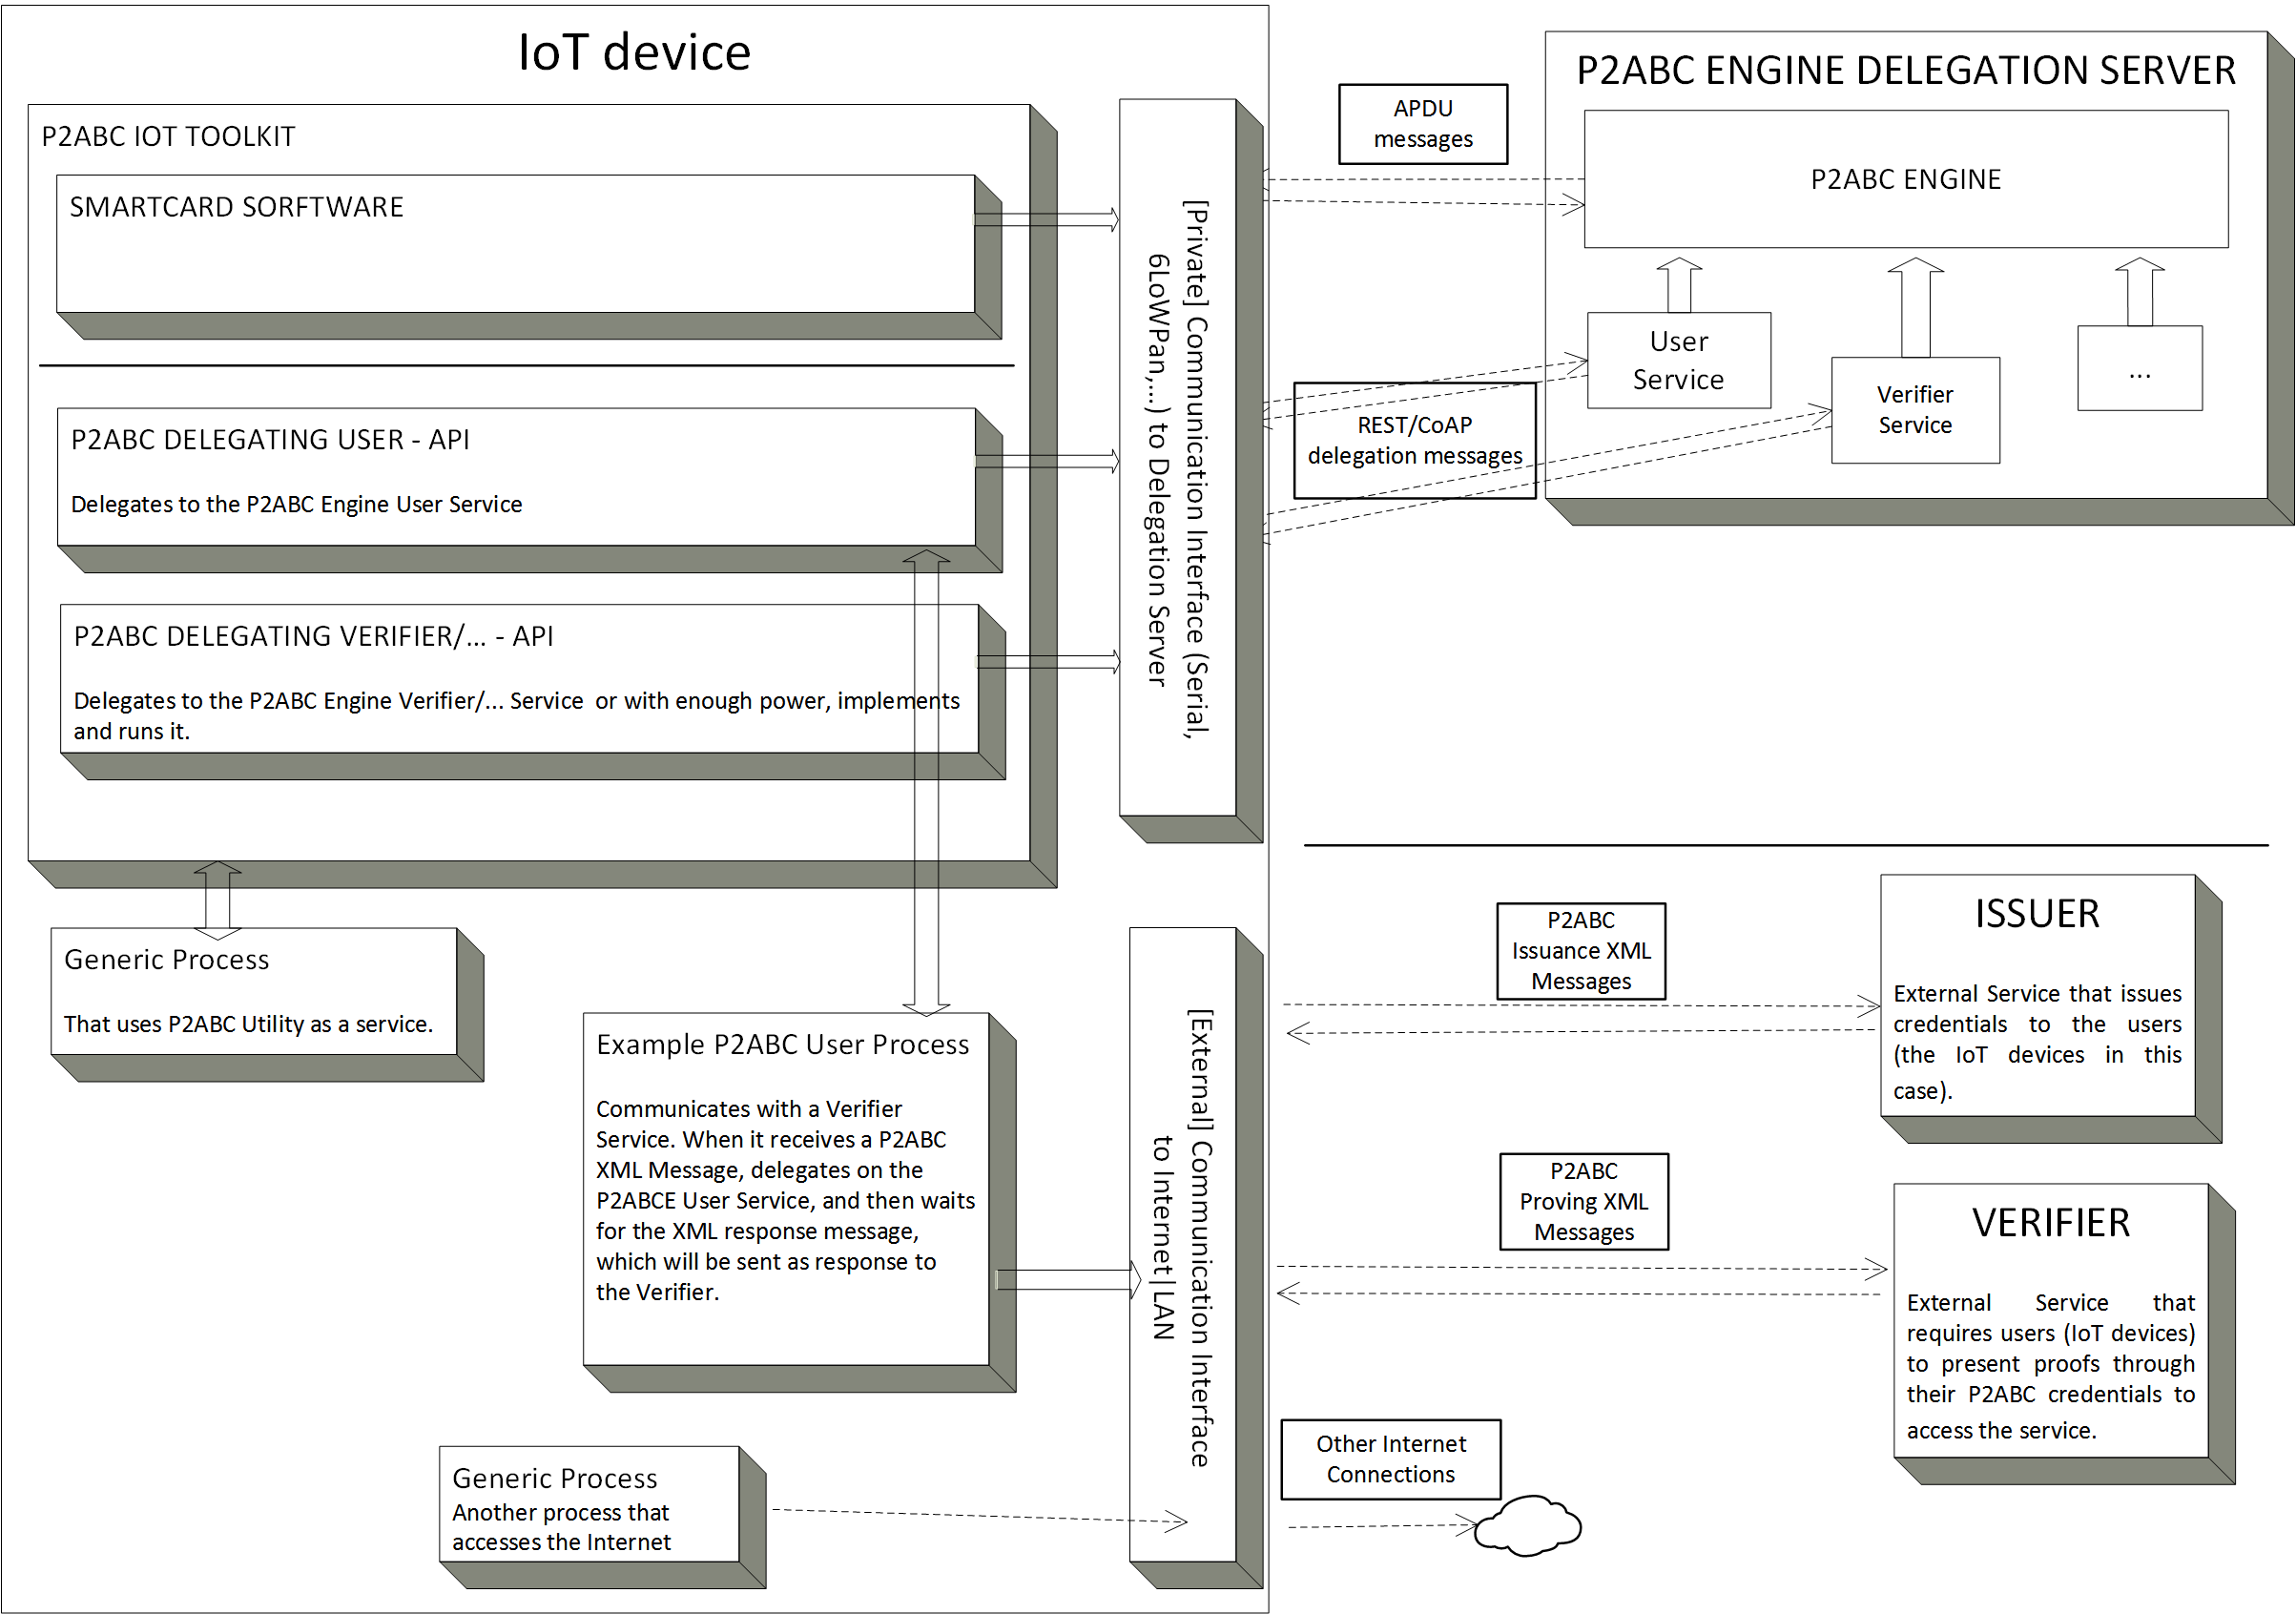
\includegraphics[width=\linewidth]{gfx/P2ABCE-IoT-bw}
	\end{center}
	\caption{IoT in P2ABCE Architecture.}
	\label{fig:P2ABCE-IoT}
\end{figure}

%\begin{figure}[bth]
%	\begin{center}
%		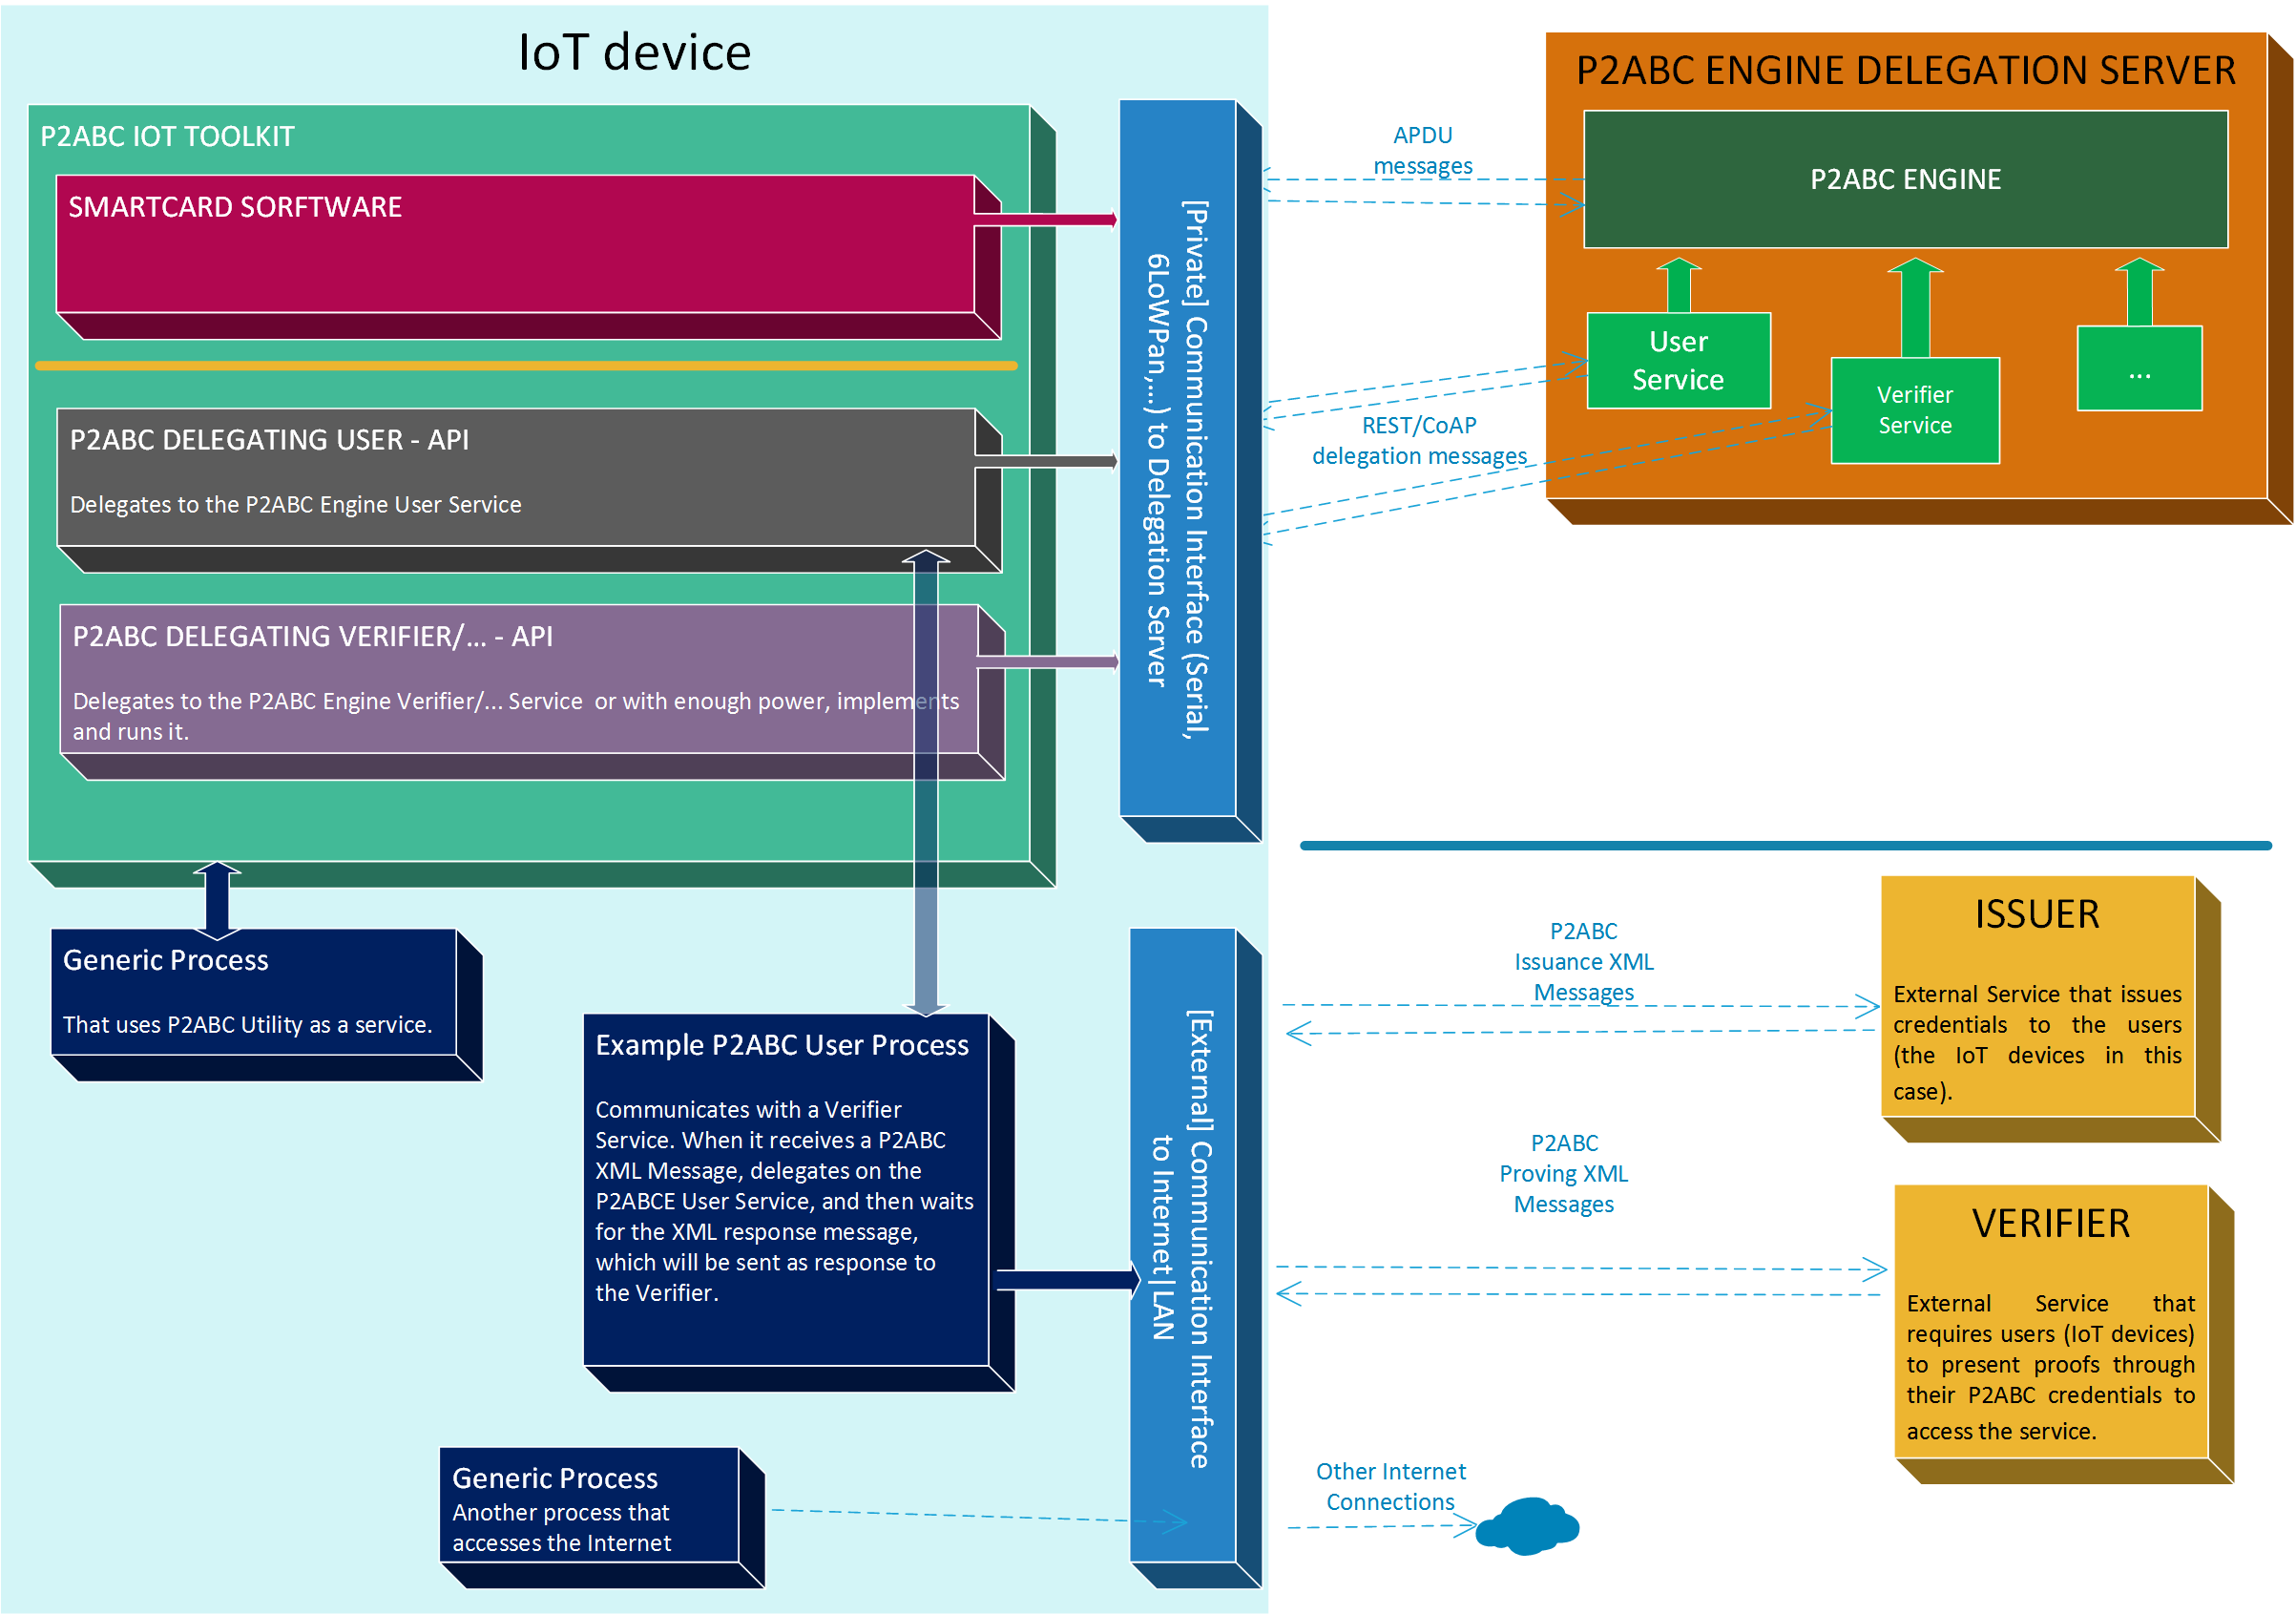
\includegraphics[width=\linewidth]{gfx/P2ABCE-IoT-color}
%	\end{center}
%	\caption{IoT in P2ABCE deployment diagram.}
%	\label{fig:P2ABCE-IoT-color}
%\end{figure}

\hfil


The system will be compounded by the IoT device, the P2ABCE delegation server and the third party P2ABCE actors.

\begin{itemize}
	
	\item \textbf{IoT device}
	
	In \autoref{fig:P2ABCE-IoT} the IoT device is represented with two interfaces, physical or virtual. One allows external communications to other machines, including other P2ABCE actors, that could be on the Internet, a corporate LAN, a M2M overlay network, etc. Through this interface, the P2ABCE XML messages are exchanged as in any other deployment. This allows an IoT device to interact with other actors without special adaptations to the protocol. The other interface allows a secure communication with the delegation server. Both the delegation messages and the APDU Dialogue are transmitted over this interface, making it a point of attack to the system, and we will talk about its security in the delegation process.
	
	The scheme also shows the \textit{P2ABCE IoT Toolkit}. This piece of software includes the IoT Smart Card, and the API for other processes that want to use the P2ABCE system.
	
	The IoT Smart Card is the implementation of a software smart card, listens for APDU Commands from the secure interface and stores securely the credentials and private keys within the device's memory.
	
	The P2ABCE API is an interface for other processes that wish to use the private-preserving environment of P2ABCE. It provides access to every operation available, hiding the delegation process. In the future, if for example the Verification Service is implemented for the IoT device, i.e., there's no need to delegate to other machine to act as a Verifier, then any program using the API won't need to change anything, the toolkit conceals the transition from delegating to native execution.
	
	
	\item \textbf{P2ABCE actors}
	
	If we recall from \autoref{analysisP2ABCE}, the possible roles in the system were the Issuer, the User, the Verifier, the Revocation Authority and the Inspector. All of them use the P2ABCE XML schema in the specification to communicate to each other. Any third party actor will be unaware of the fact that the device is a constrained IoT device that delegates on the P2ABCE server.



	\item \textbf{P2ABCE Delegation Server}
	
	The machine in charge of receiving authorized IoT devices' commands to parse the XML files exchanged and orchestrate the cryptographic operations the IoT smart card must perform.


\end{itemize}

\hfil

\begin{flushleft}
	\textbf{Delegation process}
\end{flushleft}

Here we describe the computation offloading carried out by the IoT device.  In \autoref{fig:DelegationProving} we show an example of the IoT acting as a User, Proving a Presentation Policy to a third party Verifier.

\begin{enumerate}
	\item Communication with P2ABCE actor.
	
	The IoT device starts an interaction with another actor, e.g. an Issuer or Verifier, receiving a P2ABCE XML file.
	
	
	\item Delegation to the P2ABCE Server.
	
	Depending on what role the IoT device is acting as, it will delegate in the corresponding service, e.g. User Service. The delegation message must include the XML file, and any parameter required to accomplish the task, like the information on how to communicate with the IoT smart card (listening port, security challenge, etc.).
	
	\item APDU Dialogue (if necessary).
	
	The server may need to send APDU Commands to the IoT smart card to read the credential information or perform cryptographic operations involving private keys.
	
	\item Server response.
	
	The server may return a status code or a XML file if the first one required an answer from the IoT device, in which case, it will send as response to the third party actor, resuming the communication.
	
\end{enumerate}

\begin{figure}[bth]
	\begin{center}
		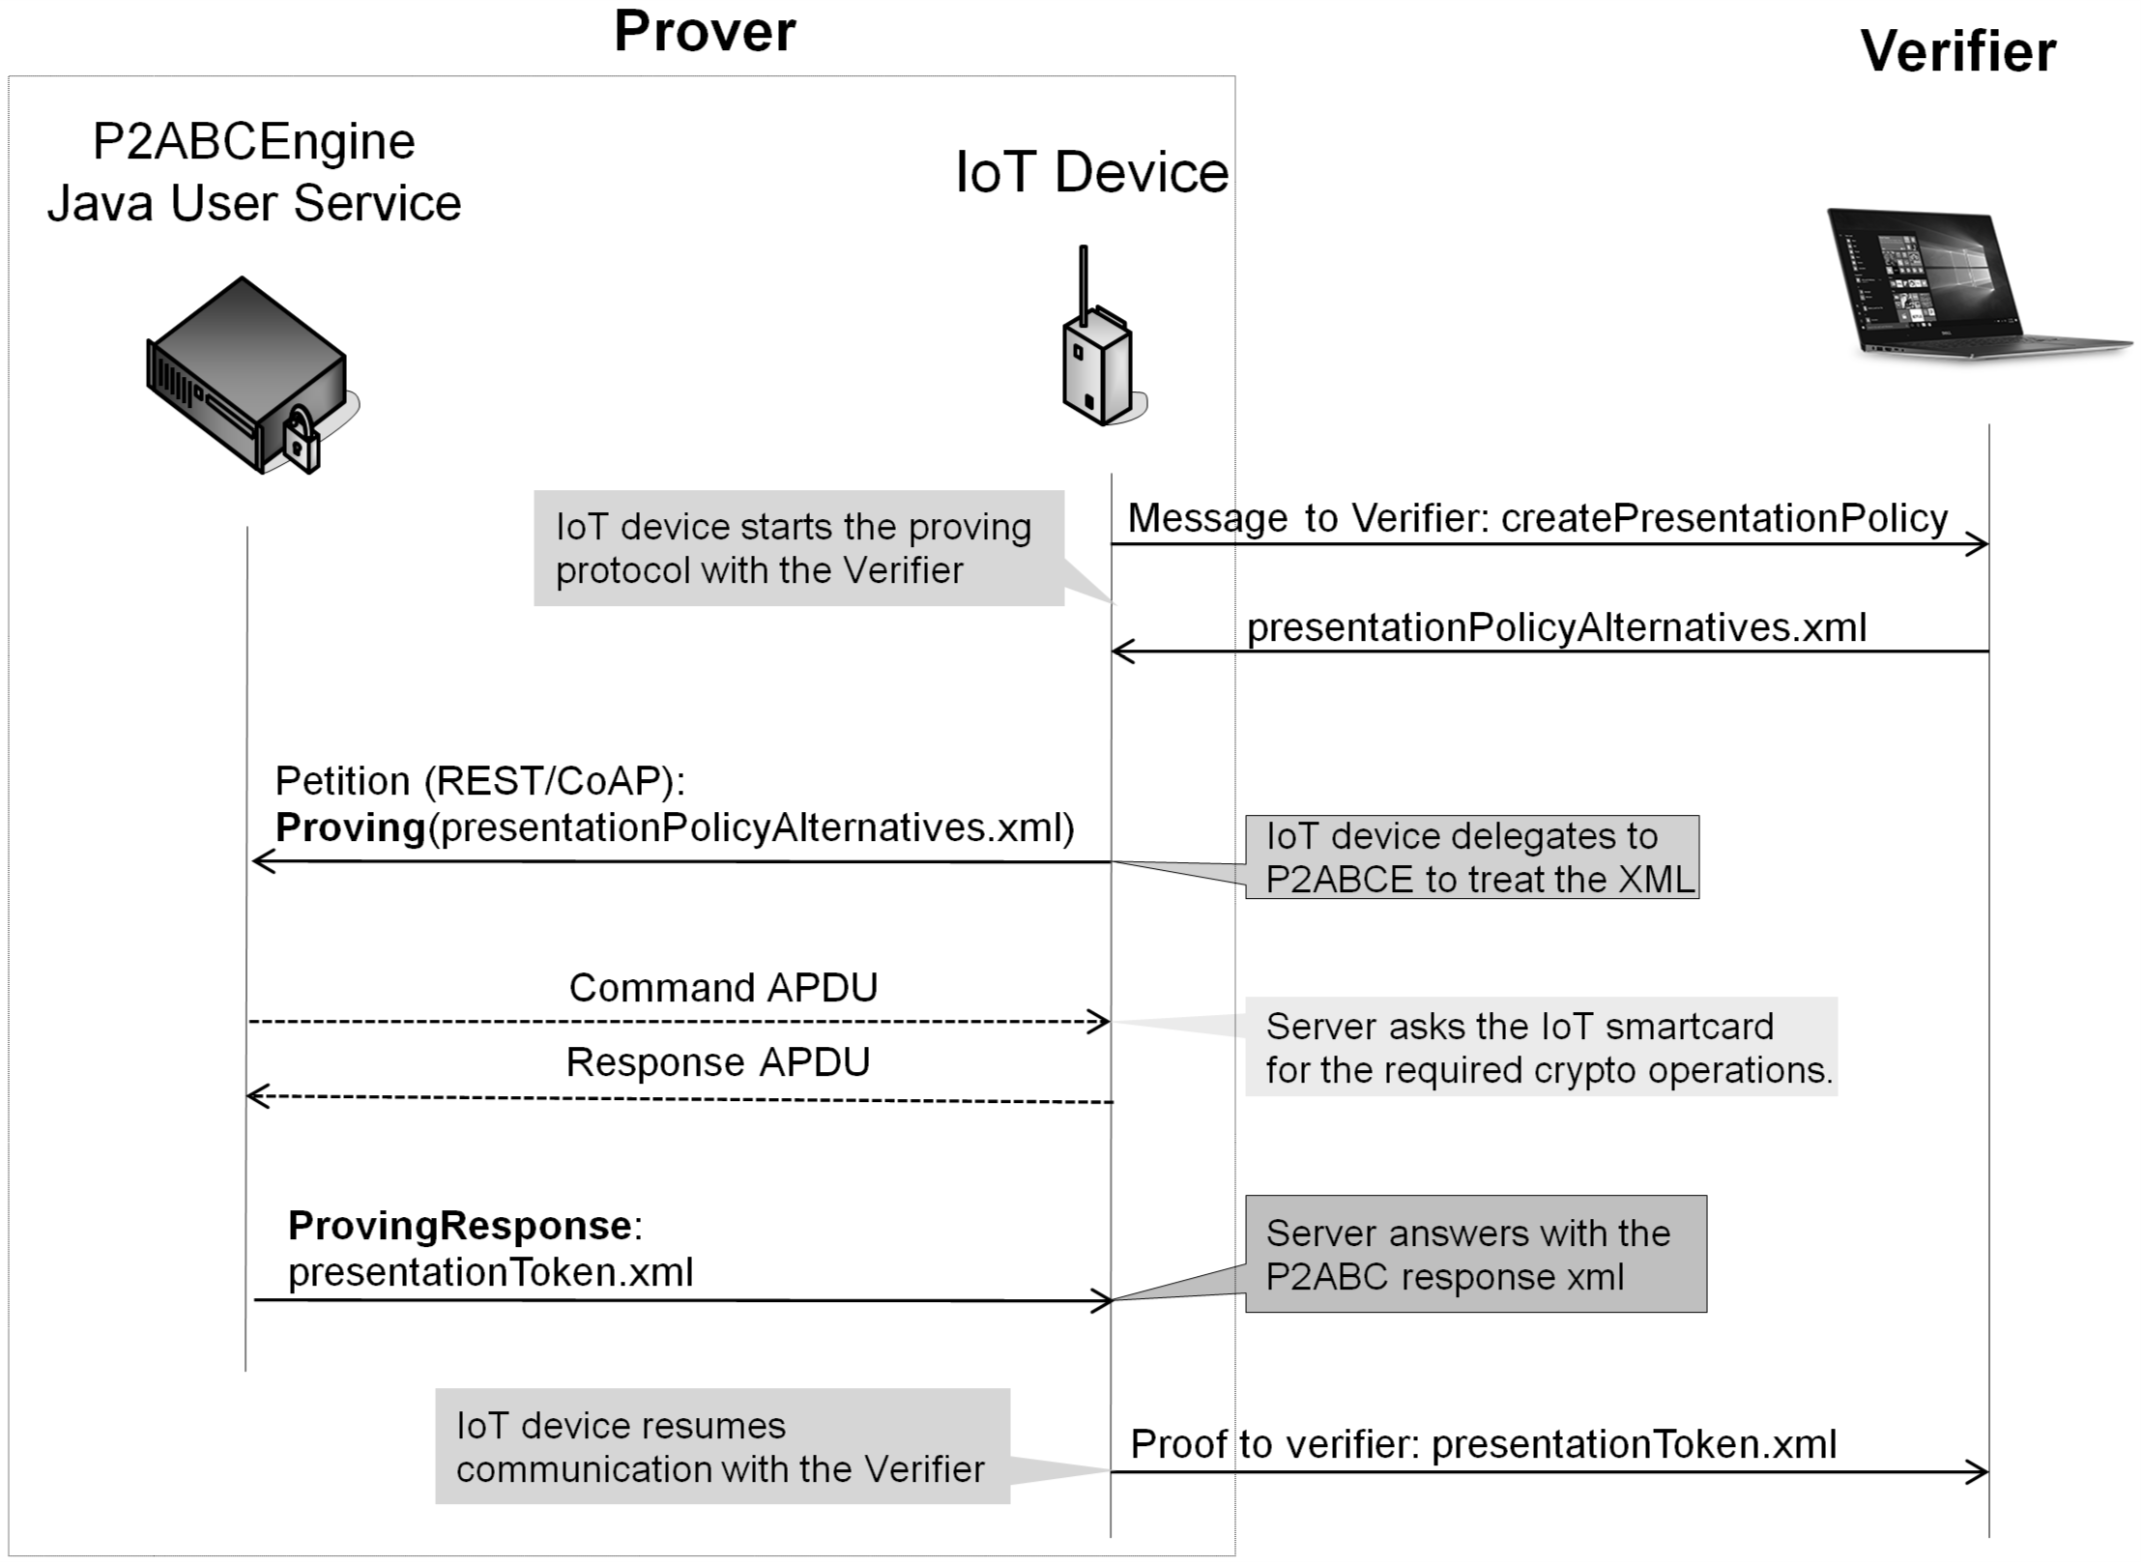
\includegraphics[width=\linewidth]{gfx/UML/DelegationProving}
	\end{center}
	\caption{IoT Delegation in P2ABCE for Proving.}
	\label{fig:DelegationProving}
\end{figure}

Transmissions over the \textit{Server-IoT} channel must be secured in order to avoid attacks like: impersonate the P2ABCE delegation server, having access to the IoT smart card sending the APDU Commands the attacker wishes; delegate as a device on the server but giving the parameters of another device, making the delegation server send the APDU Commands to a victim IoT smart card.


We could use a corporative PKI to issue certificates to the server and devices and configure policies for access control; design a challenge-response system combined with the smart card PIN, like a password and TOTP\footnote{Time-based One-time Password} in a 2FA\footnote{Two-factor authentication} login. We also could connect physically the delegation service through RS-232 serial to the IoT device, securing both physically as we would do with the IoT device on its own, isolating the delegation system from any network attack. This last idea is an approximation to the Arduino Yún\footnote{\url{https://www.arduino.cc/en/Main/ArduinoBoardYun}}, a development board that integrates two microcontrollers, one a typical Arduino with very low resources, and another one running a fork of OpenWrt. The Arduino microcontroller can control the terminal of the more powerful one, using the serial pins as commented before.

As we can see, there are many state of the art solutions for all this threads, therefore, we can assume a secure channel without mentioning a specific solution, providing freedom to choose the most fitting one in a real deployment.


\paragraph{Notes for more constrained devices}

Our architecture is designed for devices that could in a future run a reimplemented version of P2ABCE, that means, the devices could perform more tasks than only running the smart card software and their main purpose process, e.g. recollecting sensor data. But if our target devices are so constrained that can barely run the smart card, they may not be able to handle the XML files because of memory restrictions, like a MSP430\footnote{\url{http://www.ti.com/lsds/ti/microcontrollers-16-bit-32-bit/msp/overview.page}} running Contiki-OS, the microcontroller has between hundred of bytes to tens of kilobytes of memory, making impossible to store multiple XML files in the size range of tens of kilobytes.

In these cases, the delegation in the server goes a step forward, making the server a proxy to communicate with other P2ABCE actors, and the IoT device only acts as a smart card. The IoT device would still act as the User, or any other P2ABCE, role because it orchestrates when and how an interaction with other actor is executed, but the communications would be between the proxy and the third party actor. 



\section{Proof of Concept Implementation}
% +Implementation:
% *System:
% 	-Raspbian OS: distro de debian para Raspberry Pi, que se describirá en los tests
% 	-LEDE: ash terminal (shell command interpreter), POSIX, typical hardware, libraries with no hardware aceleration vs smart card MULTOS,
%
% *Delegation
%  -REST as current delegation protocol: curl script bash
%  -BIOSC as current APDU transmission protocol: no security -> no overload.
% *Smart Card
%  
%  -IoT Smart Card software design and implementation notes.
%  -Sequence diagrams. TODO


In this section we present the first PoC implementation, introducing the IoT system where we are going to work, then we will describe the delegation protocols, one for the computation offloading of the IoT device on the P2ABCE server, and another for the transmission of APDU Commands, and finally, we will describe the IoT smart card implementation.



\subsection{IoT system}

We will develop our PoC in Linux based systems in order to avoid complications with firmware specific issues that we are not familiar with. Even so, the linux systems used are aimed for the IoT environment and serve as a starting point for future implementations in more constrained devices or different systems.

In our delegation server we will run Raspbian OS, a distribution based on Debian for the Raspberry Pi. We will talk more about the hardware specifications in the benchmark chapter. We chose this system because it has a great package repository support, including the Java Runtime Environment, needed to run the P2ABCE Services.

For our IoT device, we will use LEDE, Linux Embedded Development Environment, a distribution born from OpenWrt, aimed for routers and embedded chips with low resources requirements. It offers the \texttt{ash} command interpreter, or \texttt{shell}, and the \texttt{opkg} package manager, that allows an easy installation of some libraries and tools needed during the early development.











\subsection{PoC Delegation}

As we explained in the design section, the delegation has two steps, the IoT device calling the P2ABCE server to offload the parsing of the XML data, and the P2ABCE server sending APDU Commands to the IoT smart card in the device.




\subsubsection{PoC Delegation to the P2ABCE Server}


Currently P2ABCE offers multiple REST web services to run different roles in P2ABCE system: User Service, Issuer Service, Verification Service, etc. Any third party application that integrates P2ABCE with their system can make use of these services or implement the functionality using the library written in Java, the tool that the REST services actually use.


Our PoC machine, the Omega2, can make REST calls easily with the \texttt{curl} command, but other devices may use \ac{CoAP}, but in that case, the P2ABCE REST services should be adapted to offer CoAP support. The commands needed to delegate to the P2ABCE server would be the same that those defined now to operate with the REST services, but with the modifications needed to pass the parameters on how to communicate with the IoT smart card.

In this PoC the only P2ABCE Service that needed to be modified was the User Service. We added the following REST call

\begin{center}
	\textit{/initIoTsmartcard/{issuerParametersUid}?host=\&port=}
\end{center}

where we communicate the P2ABCE server that an IoT Smart Card is accessible via \textit{host} and \textit{port}. Then a new \textit{HardwareSmartcard} object is stored in the P2ABC Engine, but instead of the \textit{javax.smartcardio} Oracle's \textit{CardTerminal} implementation, we use our own \textit{IoTsmartcardio} implementation for the \textit{HardwareSmartcard} constructor, that we will discuss in the following section.


\hfil

In a real deployment, we would offer a full library with an API for other processes that want to use the P2ABC Engine, which automatizes the boot of the IoT smart card and handles the security policies, like the one we presented in the deployment diagram \ref{fig:P2ABCE-IoT} of the \textit{P2ABCE IoT Toolkit}.

Now we show some examples of the PoC \texttt{curl} commands, run in the device's terminal, or from a shell script for automation:

\begin{lstlisting}[language=bash]
$ curl -X POST --header 'Content-Type: text/xml' "http://$DelegationServerIP:9200/user/initIoTsmartcard/http%3A%2F%2Fticketcompany%2FMyFavoriteSoccerTeam%2Fissuance%3Aidemix?host=192.168.3.1&port=8888"

$ curl -X POST --header 'Content-Type: text/xml' -d @firstIssuanceMessage.xml "http://$DelegationServerIP:9200/user/issuanceProtocolStep/" > issuanceReturn.xml
\end{lstlisting}

The IoT device will only manage XML as data files to exchange between the third party actor and the P2ABCE delegation service, attaching them in the body of the REST call. In the parameters of the first call we can see the IP and port where the IoT smart card will be listening.



\subsubsection{APDU Dialogue Transmission}


To transmit the APDU messages in our PoC we use a simple protocol, that we will refer as BIOSC (Basic Input Output Smart Card), consisting in one first byte for the instruction: 

\hfil

\begin{tabular}{|c|l|}
	\hline
	\texttt{0x01} & APDU Command or Response: Read 2 bytes for the\\& length and then as many bytes as said length. \\
	\hline
	\texttt{0xff} & Finish connection: close the current TCP socket and\\& end the IoT smart card execution. \\
	\hline
\end{tabular}

\hfil

In the first instruction, we read two header bytes with the length of the APDU Command or Response to receive, followed by said APDU bytes. The message is sent over TCP for a reliable transmission (concept of session, packet retransmission, reordering, etc.). The second instruction serves for closing the TCP socket in the IoT device when the smart card is no longer needed.

We lack any security (authentication or authorization) that a real system should implement. It is vital to authenticate the delegation service, to authorize it to make APDU Commands, and the same with the IoT device, to prevent attacks. But using this method for the transmission of the APDU messages, with only 3 bytes of overhead, helps us in the  benchmarks to measure the real performance of the system.


\hfil


The implementation of this simple protocol is done in both Java and C, one for the P2ABCE server and the other one for the IoT smart card.

\hfil

As we mentioned in the analysis of P2ABCE's code, the \texttt{HardwareSmartcard} class implements the \texttt{Smartcard} interface using the package of abstract classes \texttt{javax.smartcardio} to communicate with the physical smart cards. The Oracle JRE implements these package for the majority of smart card manufacturers. For our PoC, we implement the \texttt{javax.smartcardio} package so it transmits the APDUs with BIOSC, making the use of a physical or IoT smart card totally transparent to the \texttt{HardwareSmartcard} class, enhancing maintainability, and following the \textit{expert pattern} from the known GRASP guidelines.

%TODO : optional: diagrama secuencia de P2ABCE, pero si eso solo de la reimplementación de javax.smartcardio y su uso por HardwareSmartcard

\textbf{TODO} :  diagrama secuencia de la reimplementación de javax.smartcardio y su uso por HardwareSmartcard

\hfil


In the PoC IoT device, we implement in \texttt{BIOS.c} the \texttt{main()} function, that reads from a Json file the previous status of the smart card, and then opens the TCP socket in the $8888$ port, and loops listening for BIOSC transmissions until an $0xff$ is received. When an APDU Command is sent, it calls the APDU Handler, that we will talk about in the next section.




\subsection{IoT Smart Card Implementation}


After many design decisions in the process to adapt the original ABC4Trust Card Lite code to pure C, working on a MIPS architecture, in this section, we present the current \ac{PoC} code, most important decisions taken and the execution workflow in the form of sequence diagrams.


\hfil



\subsubsection{Code structure}


We divide the project in three different sections with the objective of enhancing maintainability, improving future changes, ports, fixes, etc.

In \autoref{fig:IoTCScomponents-bw} we show the project's structure. The first section is what could be called as the core of the smart card, the second one the interface for those tools the core needs and that may depend on the target's platform, and finally, the third party libraries, that may be empty if the interfaces implementation doesn't require any.




%\begin{figure}[bth]
%	\begin{center}
%		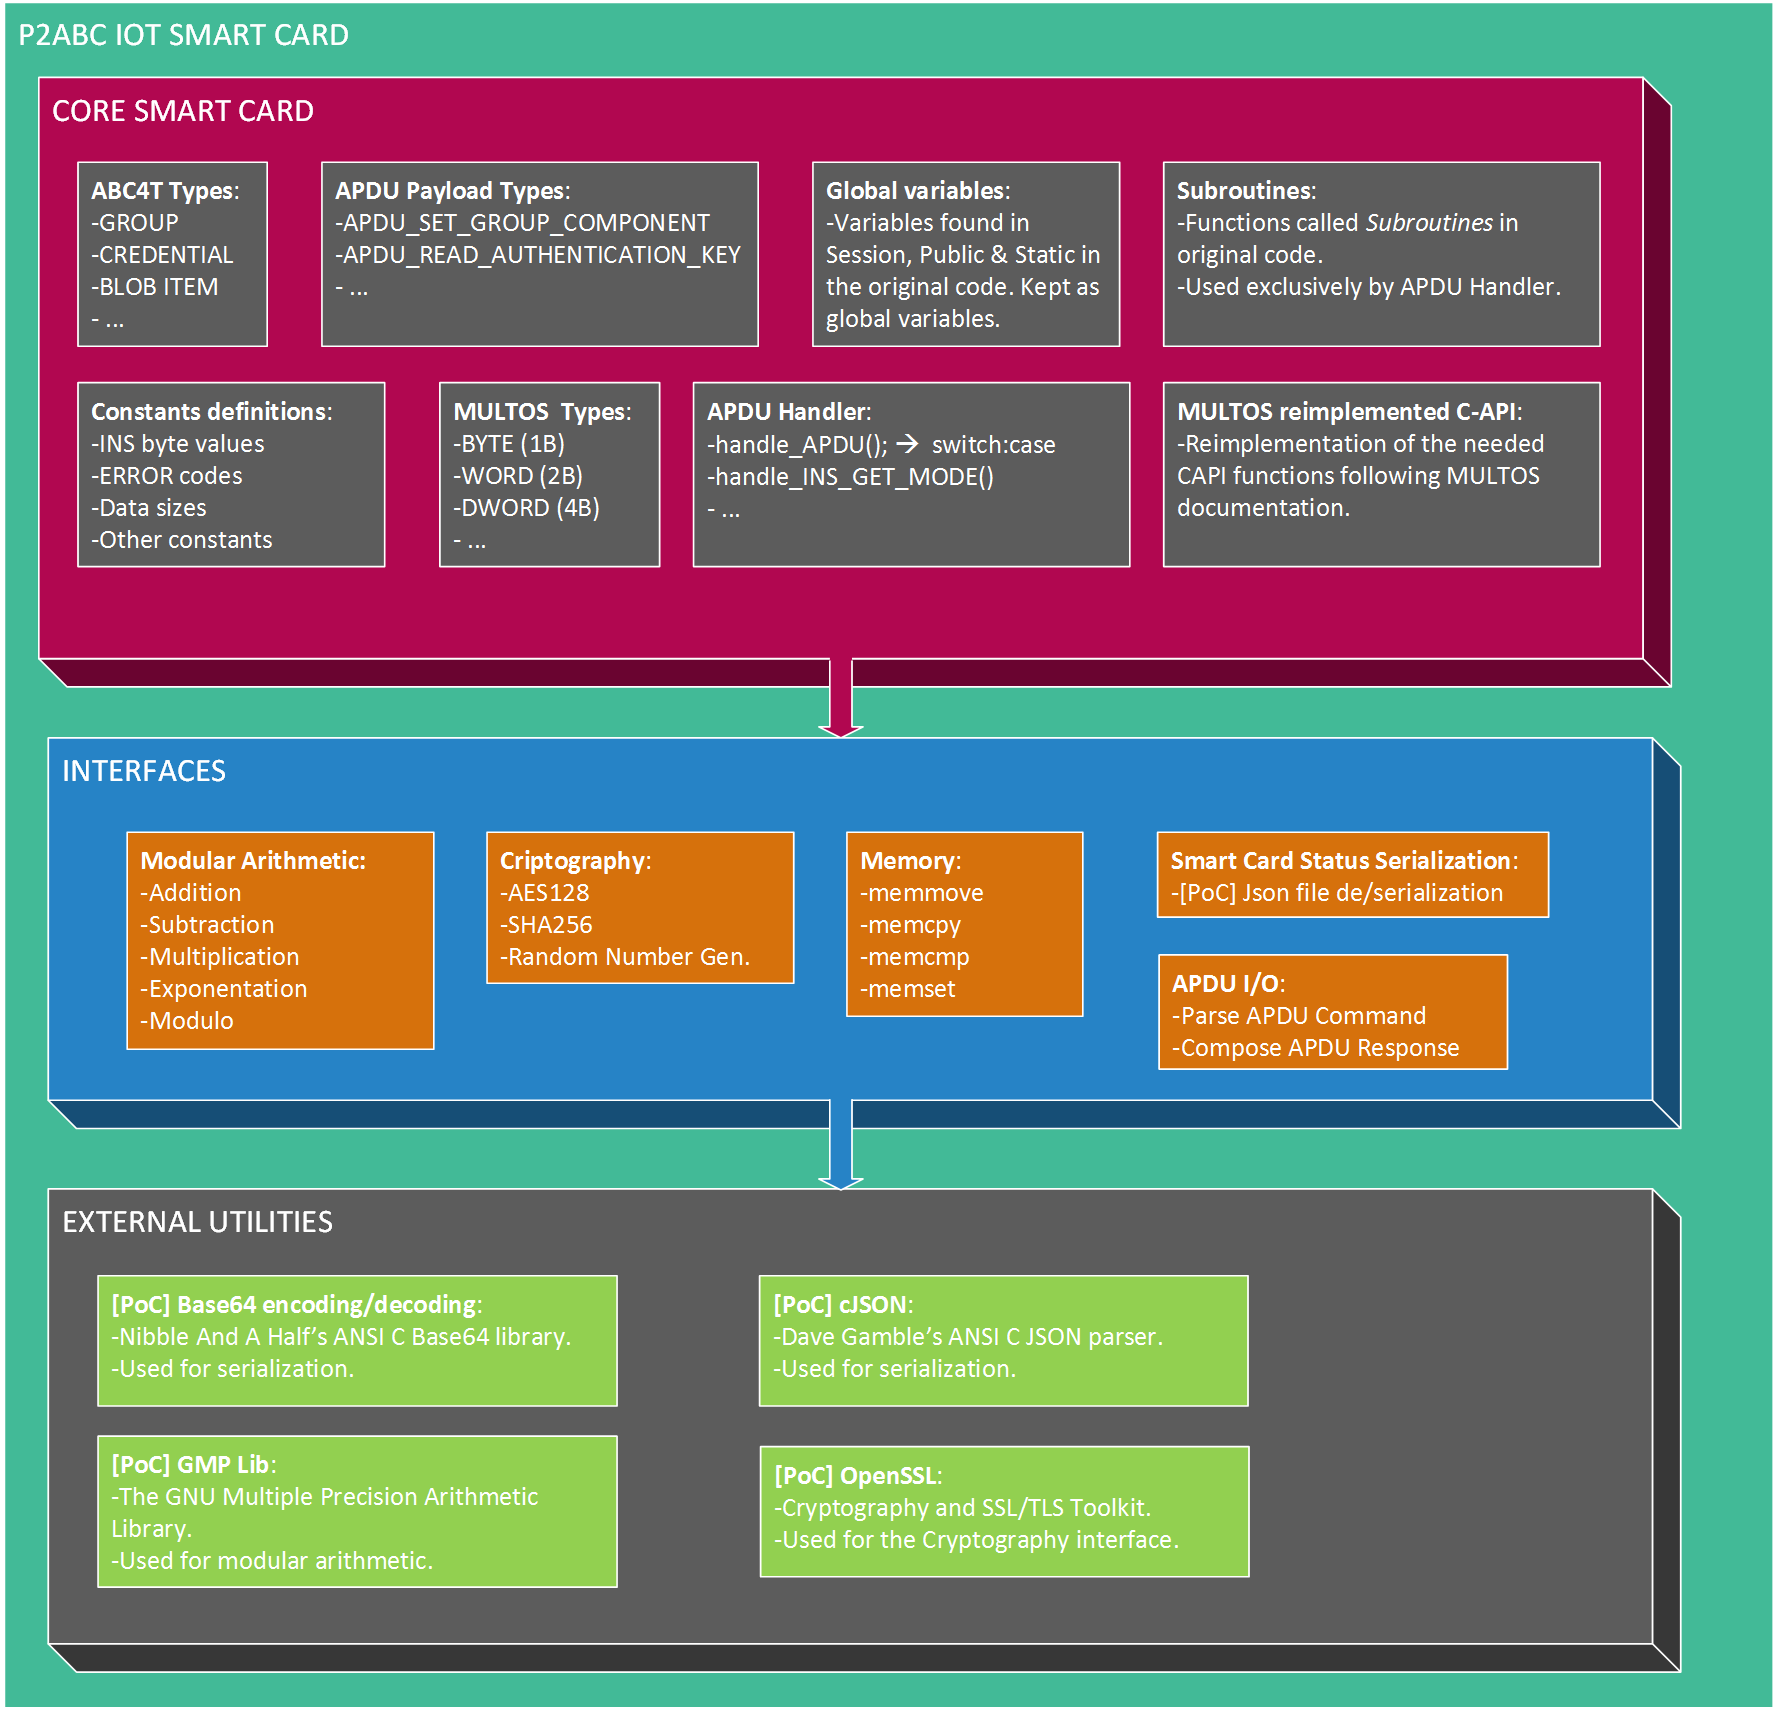
\includegraphics[width=\linewidth]{gfx/IoTCScomponents-color}
%	\end{center}
%	\caption{IoT Smart Card Code Structure.}
%	\label{fig:IoTCScomponents-color}
%\end{figure}

\begin{figure}[bth]
	\begin{center}
		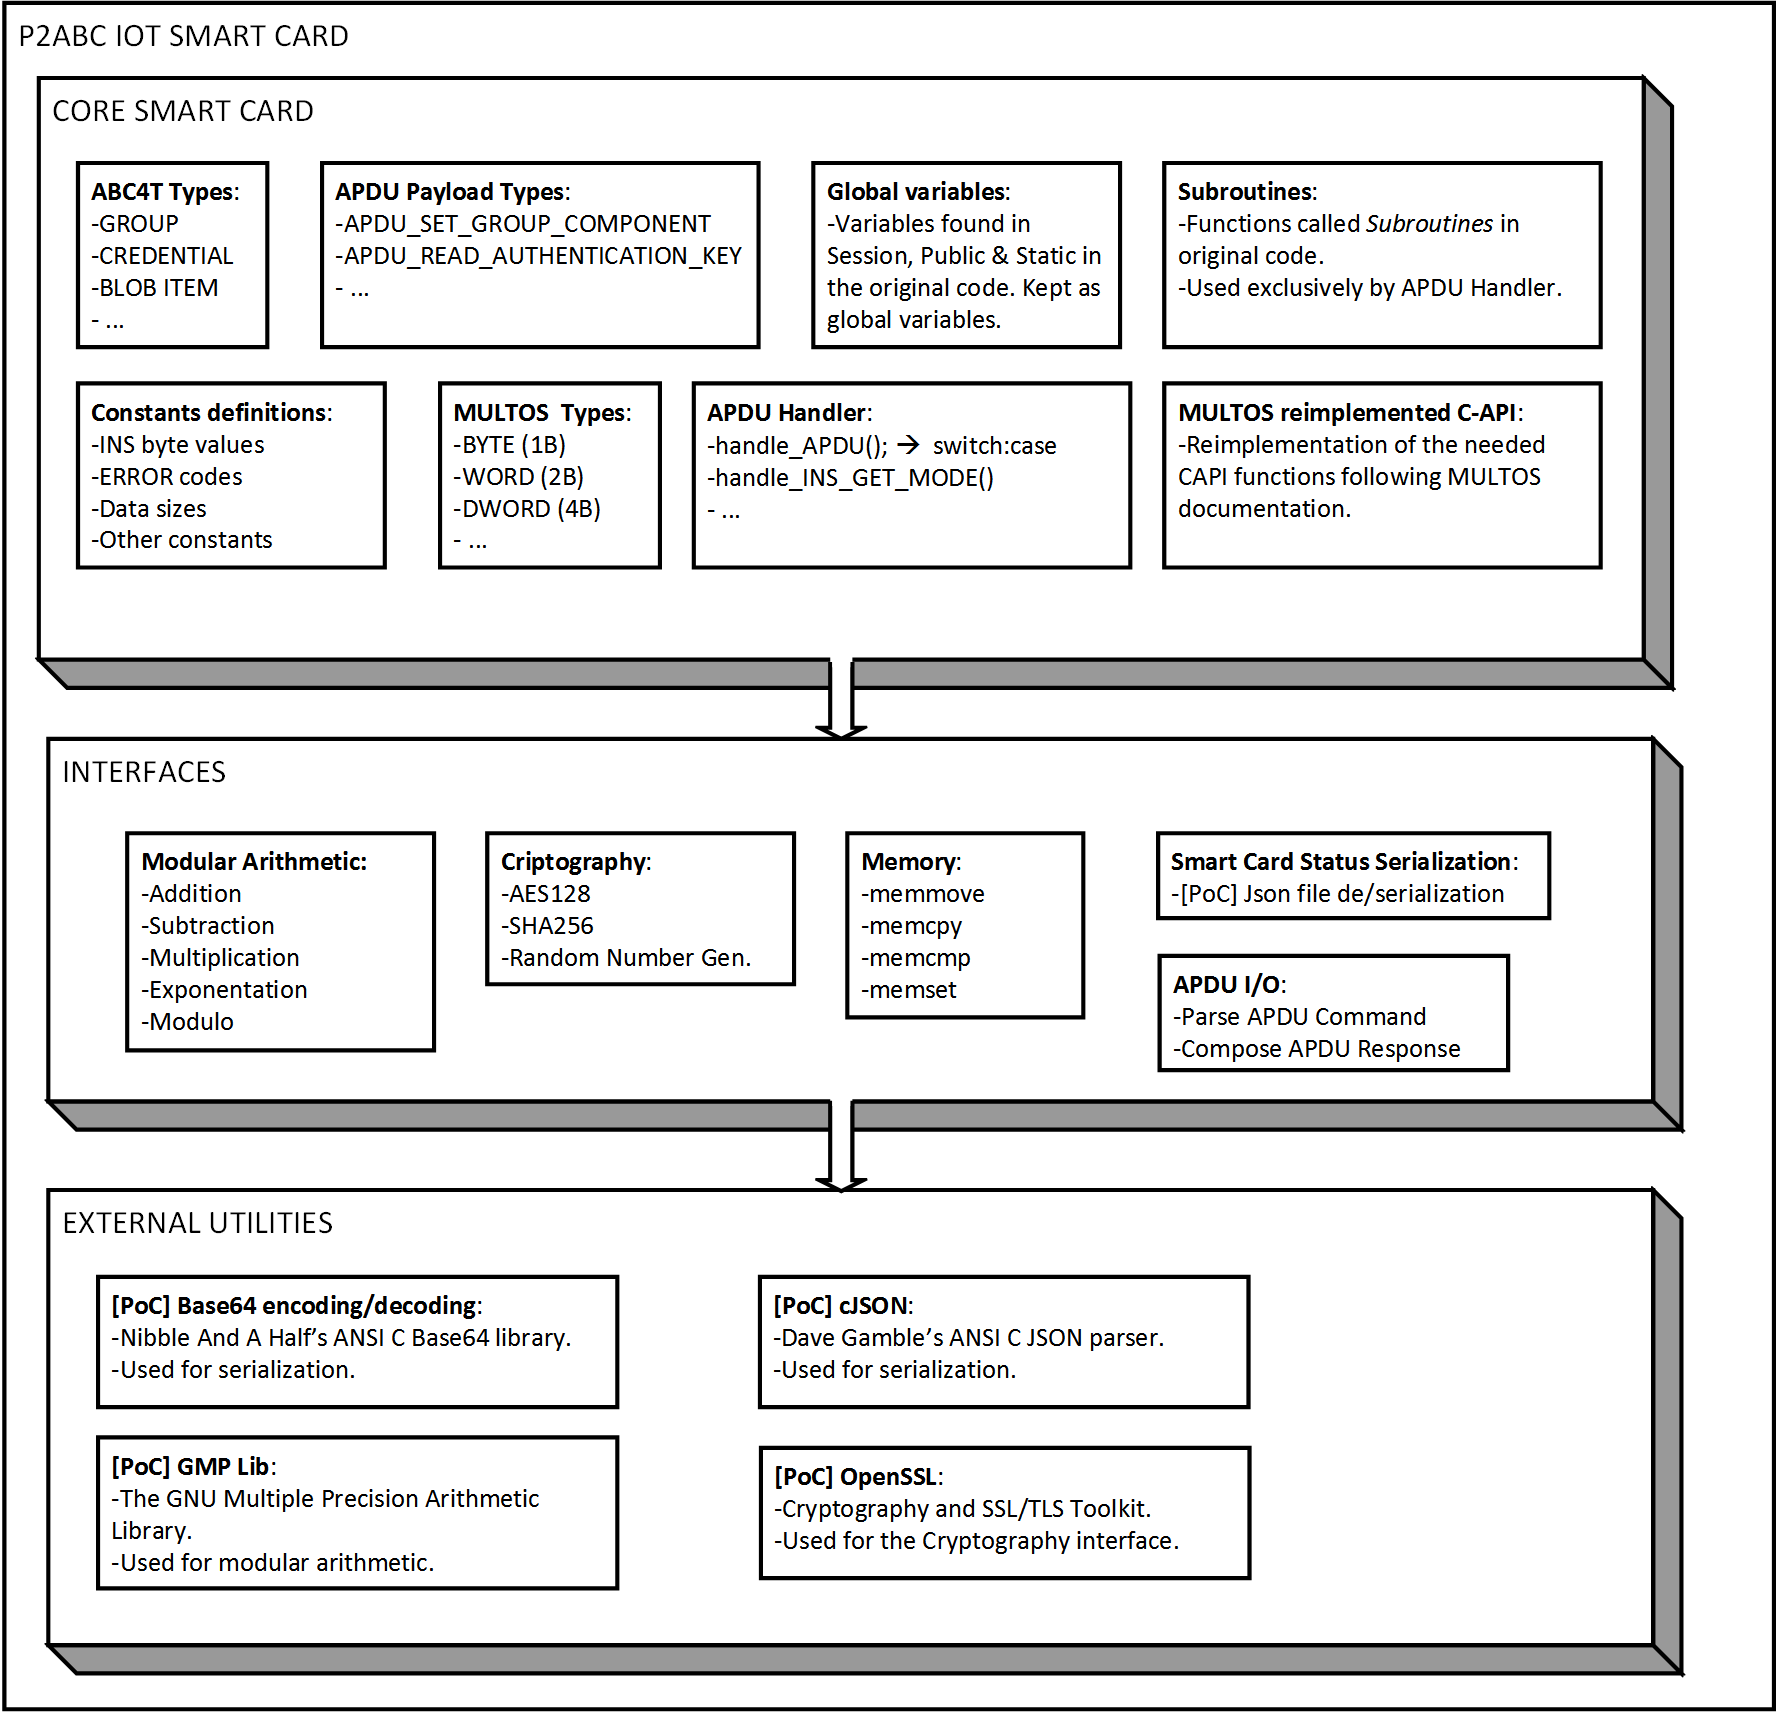
\includegraphics[width=\linewidth]{gfx/IoTCScomponents-bw}
	\end{center}
	\caption{IoT Smart Card Code Structure.}
	\label{fig:IoTCScomponents-bw}
\end{figure}


\hfil

\paragraph{Core smart card}
\hfil

The smart card logic lies in this section, the concepts of APDU Commands, what instructions are defined for P2ABCE smart cards, and how to process them and generate proper APDU Responses.

If the APDU protocol defined for P2ABCE smart cards changed, with the consequence of having to update all smart cards in use, the changes to adapt the IoT smart card should be applied in this part of the code. This also implies that if the P2ABCE Java code changes their \texttt{Smartcard} interface, something more probable, the IoT smart card will still work as intended.

Most of the original ABC4Trust Card's code has been reused in this section, e.g., all the global variables and custom data type definitions, the APDU Command handling and auxiliary subroutines.

However, the ABC4Trust's code heavily depended on the MULTOS platform for the input and output of data, modular arithmetic, memory management, and AES128 and SHA256 cryptographic operations. Therefore, we reimplement the used MULTOS functions following the documentation, adapting it in some cases.

A characteristic of MULTOS C-API is that every function name starts with ``\texttt{multos}'', so we changing their names from \texttt{multosFoo()} to \texttt{mFoo()} for readability and to emphasize that they were no longer MULTOS functions.

The \texttt{main.h} file, from the original ABC4Trust project, also implemented some functions that were equivalent to the ones available in \texttt{multos.h}. We replaced them for the standard functions in the C-API, checking that the MEL code did the same as the documentation specified. This last detail is very important, because in \citep{vullers2013efficient} they noted that MULTOS' \texttt{ModularExponentiation} function does not accept exponents larger than the modulus size, so they implemented \texttt{SpecialModularExponentiation}, dividing the exponentiation in two that MULTOS could perform. After this analysis, when those particularities appeared, our reimplementation of the MULTOS API accepts the \textit{expanded functionality}.

\hfil

Because of the inherited code, many particularities of the internals of the MULTOS platform had to be addressed. 

One was the different memory zones, where the variables in \texttt{static} were read and written directly from the secure EEPROM, defining the status of the smart card between executions. We keep those variables in RAM, but save them in a Json file, deserializing them at the smart card boot up, and serializing always before an APDU Response is sent. From the MULTOS documentation, the \texttt{static} variables are read and written atomically, and if power source is lost during any process, memory won't get corrupted. This also means that if a MULTOS smart card sends an APDU Response, every variable that had to change, is saved in the EEPROM. Our PoC uses Json for human readability during debugging, but a real deployment should apply secure reads and writes on the file, preventing data corruption and undesired access, for example, ciphering the file with a key derived from the smart card PIN. It is also desirable another data serialization method, reducing the size of the file to store in memory constrained devices.


Another of the mentioned particularities is that the MULTOS compiler does not apply padding between variables in the data structures. For example, in an X86 machine, where a \texttt{short} is stored in 2 bytes, in the following code\footnote{From \url{https://en.wikipedia.org/wiki/Data_structure_alignment}}

\begin{lstlisting}[language=C]
	struct MyData
	{
		short Data1;
		short Data2;
		short Data3;
	};
\end{lstlisting}

each member of the data structure would be 2-byte aligned. Data1 would be at offset 0, Data2 at offset 2, and Data3 at offset 4. The size of this structure would be 6 bytes. But if we defined the following structure

\begin{lstlisting}[language=C]
	struct MixedData
	{
		char Data1;
		short Data2;
		int Data3;
		char Data4;
	};
\end{lstlisting}

where a \texttt{char} is 1 byte, and an \texttt{int} uses 4 bytes, although the total bytes used are 8 bytes, the compiler will align them in memory adding padding, like if we defined the following:

\begin{lstlisting}[language=C]
struct MixedData  /* After compilation in 32-bit x86 machine */
{
	char Data1; /* 1 byte */
	char Padding1[1]; /* 1 byte for the following 'short' to be aligned on a 2 byte boundary
	assuming that the address where structure begins is an even number */
	short Data2; /* 2 bytes */
	int Data3;  /* 4 bytes - largest structure member */
	char Data4; /* 1 byte */
	char Padding2[3]; /* 3 bytes to make total size of the structure 12 bytes */
};
\end{lstlisting}



\hfil


In MULTOS, to reduce the memory usage, there is no padding, and this affects the inherited ABC4Trust's code because of the use of \texttt{memcpy} to copy zones of memory from one address to another. The problem is the code copies multiple variables in one \texttt{memcpy} call, because, for example, the APDU Command payload includes multiple data, and instead of copying one variable at a time, the \texttt{struct} is defined with the same order and copies everything at once.

An example taken from the parsing of instruction \texttt{SET\_PROVER}:

\begin{lstlisting}[language=C,frame=tblr]
typedef struct
{
	BYTE prover_id;
	unsigned int ksize;
	unsigned int csize;
	BYTE kx[MAX_SMALLINT_SIZE];
	BYTE c[HASH_SIZE];
	BYTE proofsession[PROOFSESSION_SIZE];
	BYTE proofstatus;
	BYTE cred_ids[NUM_CREDS];
	BYTE cred_ids_size; // also called 't' in the documentation
	BYTE exists;
} PROVER;
/*****/
PROVER provers[NUM_PROVERS];

/*****/
case INS_SET_PROVER:
  // [...]
  memcpy(&(provers[temp_prover_id-1].prover_id), &(apdu_data.set_prover_in.prover_id), 5); // under the hood, this also initializes ksize and csize
\end{lstlisting}
This is the only case where a comment showcases that it is copying more than one byte.

The temporal solution is to use \texttt{struct \_\_attribute\_\_((\_\_packed\_\_))} to ask a GCC compiler to not use padding in the structs, but this is not standard, neither a good practice. A deeper refactorization of the code is needed where the hidden copies of variables are made explicit, letting the compiler manage the memory layout.


\hfil

An internal alarm should always warn us when we see raw memory copy from serialized data, that is, the APDU Payload. We mentioned in the MULTOS introduction that the platform is Big Endian. The serialized data is also typically represented in Big Endian, and our APDU Payloads do so. In our code we added a new Subroutine to check whether the device is Big or Little Endian, and to rectify the Endianness from those variables, with 2 or more bytes (the only ones affected by the Endianness), copied from or written to APDU Payloads.


\hfil


Finally, we must talk about the \texttt{multosExit} function. In a MULTOS application, to finish the execution and send the APDU Response, the programmer can call in any moment to \texttt{multosExit}, and the MULTOS OS will continue the execution, not returning to the application again.

Think about how we all have, at least once, used an \texttt{if} and \texttt{return} to avoid the \texttt{else}, like in this example:

\begin{lstlisting}[language=C]
if(condition)
	return a;
return b;
\end{lstlisting}


The use of \texttt{multosExit} in ABC4Trust code is similar, but used in almost every function. This leads to a sequence execution with many possible interruptions, leaving a full stack behind with \textit{un-returned} function calls, i.e., parameters stored in memory after a function call that never returns. In MULTOS, this memory won't affect future executions, because with the next APDU Command, the stack will be loaded with the clean application, and the Session memory stays untouched between APDU Commands, during an APDU Dialogue. 

To adapt the code, the reimplemented \texttt{mExit} function can not end the program execution, because we would lose the variables in RAM needed during the APDU Dialogue, as well as that the TCP socket would close. The solution is to refactor every use of \texttt{multosExit} in a way that, if it is called from a Subroutine, the function returns a success or error code, and the only functions that can call \texttt{mExit} are the ones handling an specific instruction.

Nevertheless, there is one exception, the \texttt{output\_large\_data()} Subroutine, which is a tool to send large data payloads without Extended APDU support. We talked about this in \ref{subsec:APDU}, mentioning the special instruction \texttt{GET RESPONSE}.

Summarizing, every Subroutine must return from its execution, as well as every instruction handler, which must call either \texttt{mExit} or \texttt{output\_large\_data()} before returning. After the instruction has been handled, the execution returns to the listening loop of BIOSC.



\paragraph{Interfaces}\hfil

To reimplement some of the MULTOS functions, we needed to use some libraries, so we defined a facade to isolate the implementation of the core smart card from our different options, that could vary depending on the hardware or the system used by the IoT device.

The use of a facade lets us, for example, change the implementation of modular arithmetic with a hardware optimized version, or a future more lightweight library, or our very own software implementation using the same data types that the core uses, minimizing the data usage.

Taking a step forward, we make the core smart card totally independent of any library, only dependant of our interfaces. This means that typical C libraries, like the standard \textit{stdlib.h}, or  \textit{string.h} are also behind the facade, in case some IoT system doesn't support them. The main goal we go after with this decision is that future developers adapting the code to a specific platform need to make no change to the \textit{core smart card}'s code, only to the interfaces implementation.

The interfaces defined can be organized in 5 groups (see \autoref{fig:IoTCScomponents-bw}), depending on their purpose: Modular Arithmetic, Cryptography, Memory Management, Serialization, APDU Parsing.


\paragraph{External utilities}\hfil

If the IoT system offers well tested libraries that could aid in the interfaces implementation, for example, a assembly optimized code for the AES128 and SHA256 operations, these third party libraries belong to this section.

In our PoC, we use two ANSI C libraries, for base64 and JSON, and two shared libraries available in as packages in LEDE, GMPLib and OpenSSL. These libraries use dynamic memory and offer more functionality than we need, although they are a good tool in this PoC, future versions should use more lightweight solutions.

For example, Atmel's ATAES132A\footnote{ATAES132A 32K AES Serial EEPROM  Datasheet - \url{http://ww1.microchip.com/downloads/en/DeviceDoc/Atmel-8914-CryptoAuth-ATAES132A-Datasheet.pdf}}
\marginpar{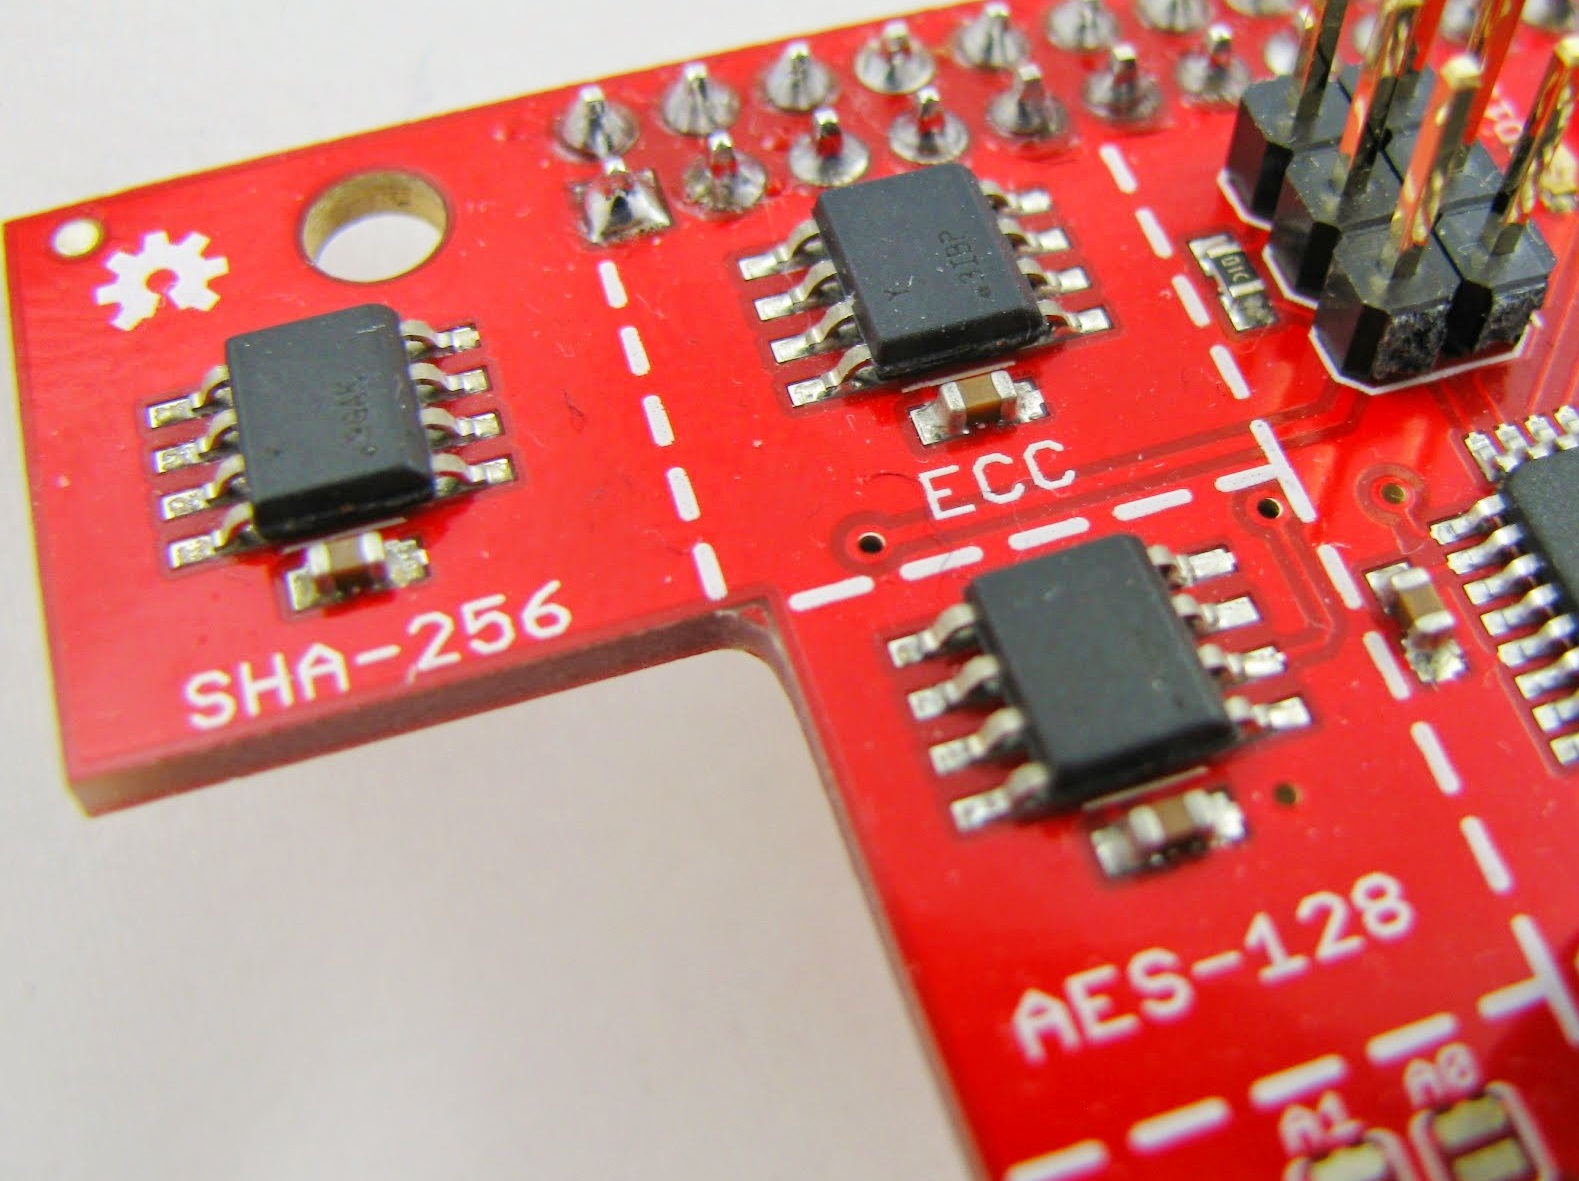
\includegraphics[width=0.9\linewidth]{gfx/atmel} \\ Atmel's cryptography chips.}
offers a serial chip for secure key storage, AES128 execution and random number generation. Another serial chip like ESP8266 offers WiFi connectivity, typically used with Arduino, and can also perform AES encryption. For random number generation, a technique used with Contiki devices is to read from sensors aleatory data and use it as seed.

All these alternatives depend on the target device, but are all valid, and would substitute OpenSSL with only a Serial communication library, so we can talk to the dedicated chips.

\hfil

The \textit{interfaces} and \textit{external utilities} sections  allow that the project is easily ported to specific targets without modifying the smart card logic.



\subsubsection{Execution workflow}

The sequence diagram from \autoref{fig:sequenceBIOSC} shows the execution of the PoC IoT smart card.



\begin{figure}[bth]
	\begin{center}
		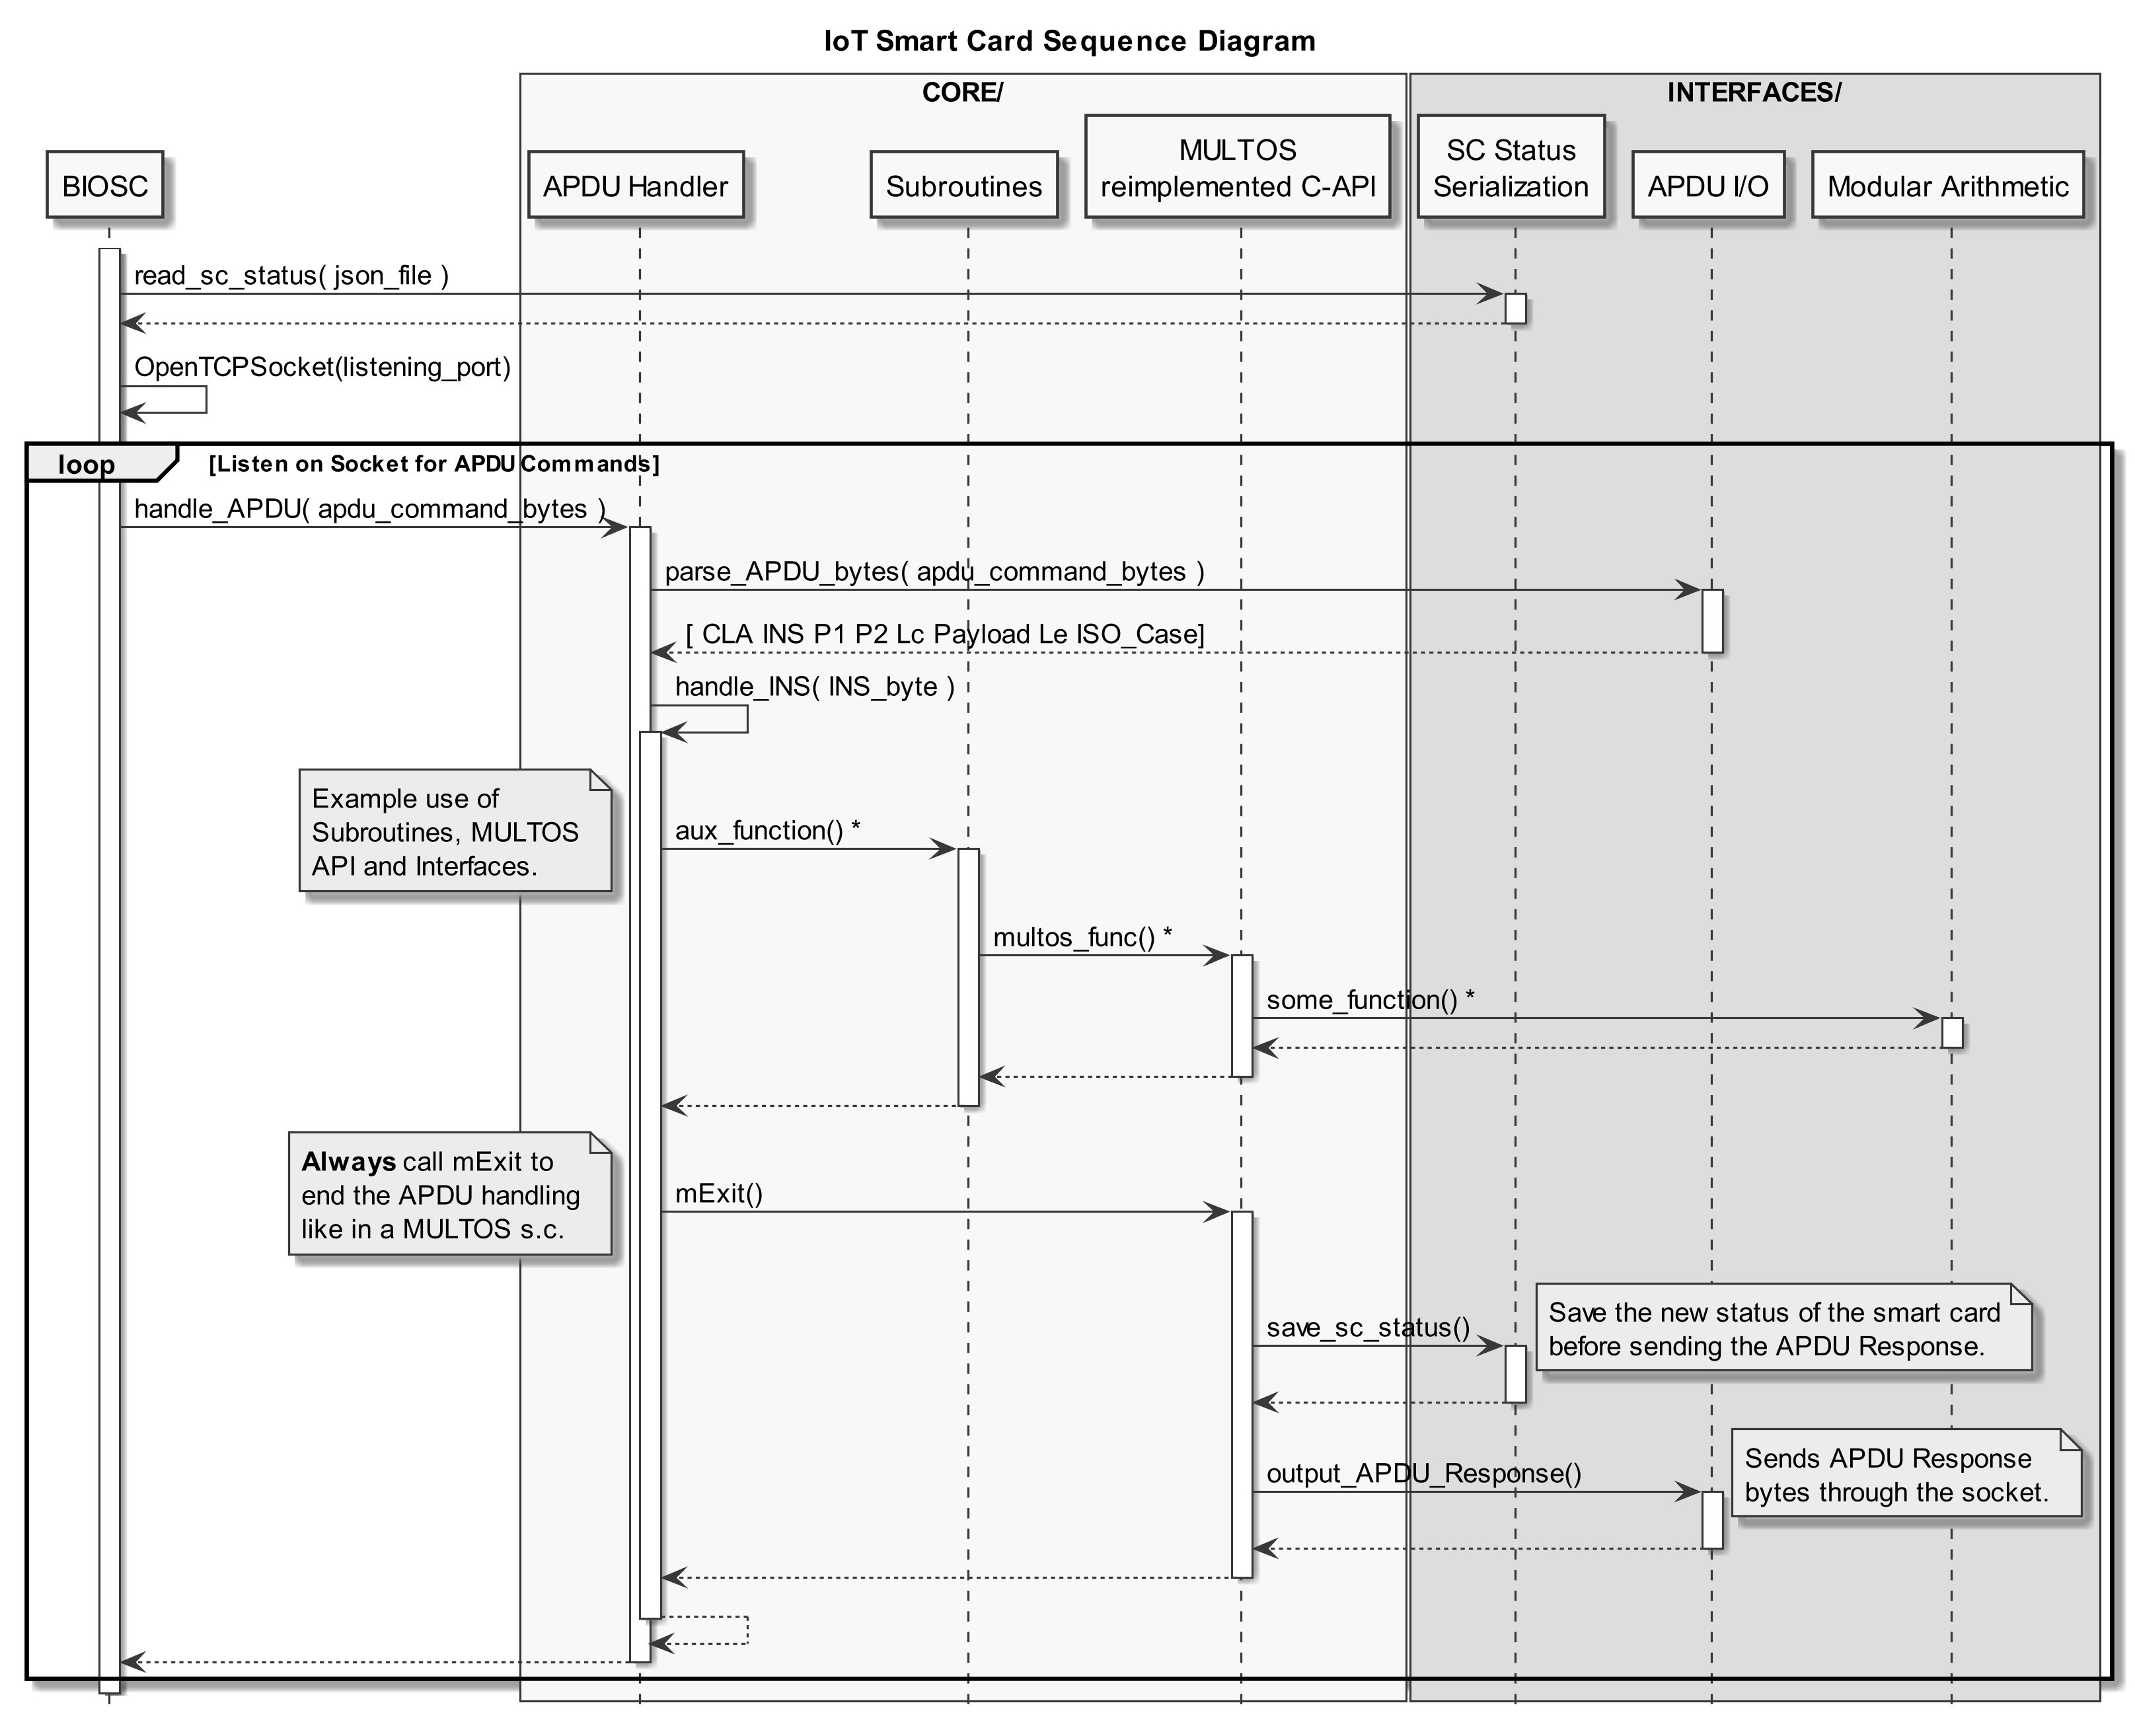
\includegraphics[width=\linewidth]{gfx/UML/sequenceBIOSC}
	\end{center}
	\caption{IoT Smart Card Sequence Diagram.}
	\label{fig:sequenceBIOSC}
\end{figure}



The program starts with the \texttt{main} function in BIOSC, that deserializes the status from the Json file, and listens on a loop for APDU Commands from the delegation server.

Every time an APDU Command arrives, it calls the function \texttt{handle\_APDU()} with the raw APDU bytes. The Handler calls the APDU I/O interface to parse the bytes, storing in global variables the APDU structure. Using a \texttt{switch-case} expression on the \texttt{INS} byte, the Handler calls an \textit{Instruction handler} function.

Inside this function, it may call multiple functions from the Subroutines, that may call MULTOS C-API functions, Which in turn may use an interface to perform its functionality.


As we mentioned, every instruction handler must end, before the \texttt{return;} expression, with \texttt{mExit} or  \texttt{output\_large\_data()}, that will use \texttt{mExit}. This reimplemented MULTOS function will save the current status of the smart card, with the help of the serialization interface, and once the file is saved, it outputs the APDU Response back to the delegation server.

After returning from \texttt{mExit}, the instruction handler and the APDU handler functions, the program listens again from the socket, until an $0xff$ byte is received.








